% Introduction to the core concepts of physiology and the book
\chapter{Introduction}\label{chp:introduction}
%\addcontentsline{toc}{chapter}{Introduction}
Updated on \today
\minitoc

This chapter introduces basic concepts for knowing and applying clinical physiology in physical therapy practice. First, it covers what is meant by clinical physiology. Second, it reviews the basic concepts of physiology. 

\vspace{5mm}

\textbf{Objectives include:}
\begin{enumerate}
    \item Explain a muscle centered approach to clinical physiology for the practice of physical therapy
    \item Provide an example of a model that is useful in physical therapy practice.
    \item Explain the basic concepts of physiology
    \item Explain how whole system function and capacity relates to multi system function and capacity. 
    \item Provide an example of how each basic concept of physiology applies to the analysis of patient/client problems.
    \item Explain the hierarchy of adaptation and adaptability from genetic, epigenetic, anatomic, physiologic, behavioral and cultural and its relevance in physiological adaptation.
    \item Explain how the International Classification of Function (ICF) clinical physiology relates to the hierarchy of adaptation and muscle centered approach..
\end{enumerate}

\subsection{A note about objectives}

Each chapter has objectives that include specific behavioral terms. There is an ordered relationship between the behavioral terms that represents increasing and nested expectations. 

To define is to understand the words being used, to know what they represent. Whether you can define something can be tested with a straightforward question such as identifying the correct definition from a set of definitions; whether you can write the definition; respond true or false to a proposed definition for a term; or identify the correct term from a set of terms when presented with a definition. 

To explain something goes beyond defining. It also implies that you can define the required terms. Explaining is the act associated with understanding. If you understand something you can explain it. Objectives are typically written as acts - what the person learning can do if they have achieved the objective. Since understanding is observed as an act of explaining, we will use the objective "explain" when there is something you must "understand". How do you demonstrate that you understand? You explain whatever it is that you understand. To explain you simultaneously hold a set of definitions together including their relationship to one another. You can explain a model by demonstrating that you know all the definitions involved, and describe how they relate to one another, and can communicate that explanation. Whether you can explain something can be tested by asking about several aspects of what you are to explain or asking you to infer which part is missing; or by asking about one part and asking you to infer the other part. The point is, to explain goes beyond defining and has an expectation of definition. But to define does not require you to explain. 

To evaluate something requires you to make judgements and to infer beyond the thing you are asked to evaluate. To evaluate implies that you can define and explain the thing (or concept) you are asked to evaluate. Being tested for whether you can evaluate can include asking you to infer to or from something that has not been directly covered or discussed, going beyond the thing (or concept)\footnotemark{}\footnotetext{By a "thing" we intend a particular thing, perhaps a particular object, whereas by a "concept" we intend a universal that will contain many particulars. For example, there is a muscle fiber as a thing, meaning this particular muscle fiber and there is the concept of muscle fiber, meaning anything that has the properties of being a muscle fiber, hence universal and conceptual. This idea of the particular (concrete) and the universal (abstract) is an important concept in and of itself for your practice as physical therapists. You have both a particular patient, perhaps Sean, and you have universal patient, perhaps everyone with heart failure.} you are asked to evaluate to consider its implications in different situations. Providing an example is an objective based on a specific task and is considered a form of asking you to evaluate since it goes beyond a particular thing (or concept) to a totally new thing (or concept). Asking you to provide an example of a model requires you to know the concept of a model well enough that you can use your background knowledge to come up with something you're already familiar with that fits what you know about models. That level of knowledge requires you to evaluate a model because you evaluated your background knowledge and determined that it is a model. The chapter objective above that asks you to provide an example of a model that is useful to physical therapy practice assumes you will be able to define, explain and evaluate the concept of a model, and that you have background knowledge about physical therapy practice that you can use to evaluate models used in practice to consider what those models are and whether they are useful. 

\section{Clinical Physiology}

Clinical physiology focuses on physiology relevant to understand health and "un" health (injury, illness, disorder, dysfunction, disequilibrium). This is a clinical physiology text for physical therapists. Since physical therapists are movement specialists, and since the physiology of muscles is integral to the movement system, the approach to clinical physiology is a muscle centered approach.  A muscle fiber\footnotemark{}\footnotetext{Muscle fibers are muscle cells, and muscle cells are muscle fibers. We do our best throughout the book to refer to muscle fibers, but if we refer to a muscle cell please know that this equates to saying muscle fiber. Similarly, when we talk about the general biological properties of cells, please know that these properties are true for muscle fibers} is a system, and muscle fibers are the structural unit of muscle. 

A muscle fiber creates tension. It interacts with other systems and is supported in order to create tension. Clinical physiology for a physical therapist considers muscle tensioning, what and how a muscle fiber interacts with other systems, and what support is required for the muscle fiber to create tension.

Muscle fibers create tension for the purpose of generating movement. To create tension muscle fibers interact  with other fibers and are supported by other systems. Interactions and support are an important part of the book. Muscles get a lot of their support from the the extra cellular fluid (ECF), and maintain their ability to create tension through cellular and structural integrity.

Clinical physiology for physical therapy considers the three interactions depicted in Figure \ref{fig:muscle_centered_approach}. These interactions are supporting relationships. The interaction between the muscle fiber and movement is an undeniable part of the movement specialist’s domain of knowledge and physical therapy students have little problem understanding its importance. The relationship between the extra-cellular fluid and the muscle fiber, and between movement and the extra-cellular fluid are less obvious and deserve additional explanation. The following sections explain these supporting interactions.

\begin{figure}[!ht]
    \centering
    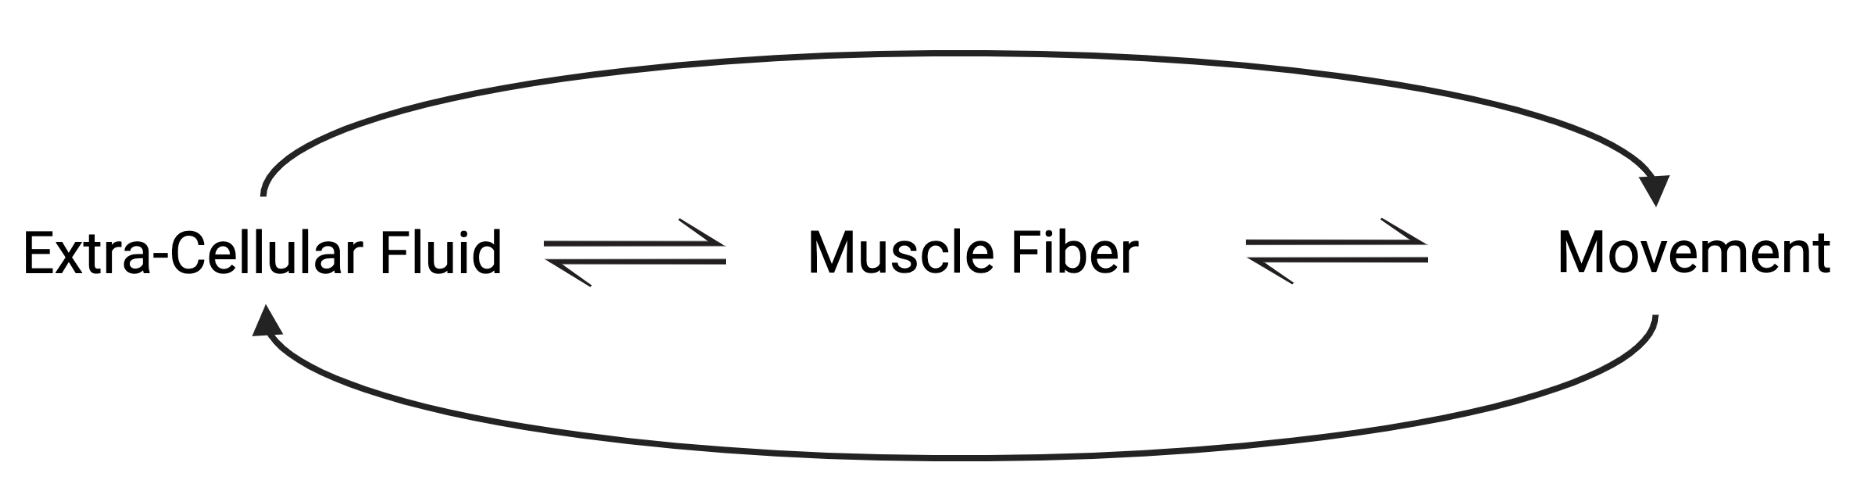
\includegraphics[width=1\linewidth]{./figure/muscle_centered_approach.png}
    \caption{A Muscle Centered Approach \footnotesize{(Created with BioRender.com)}}
    \label{fig:muscle_centered_approach}
\end{figure}

\subsection{Muscle Fibers \& Movement}

Muscle fibers are necessary but not sufficient causes for human movements. Movements include an intricate combination of active and passive tension that is created by muscle fibers. However, muscle fibers cannot create tension for movement in isolation.  First, muscle fibers must come together as a muscle and combine their ability to create tension in order to create movement. They create tension with interaction to attachments, mostly, to bones\footnotemark{}\footnotetext{Mostly to bones because sometimes muscles attach to something other than bones such as the eye muscles or facial muscles that attach to skin to create facial expressions, or muscles that attach to themselves.} that form joints that are capable of movement. The process of coming together, and creating tension and transmitting tension to bones is covered in the next two chapters (Chapter \ref{chp:fundamentals} on Fundamentals \& Chapter \ref{chp:tension} on Tension). Other aspects of movement such as the mechanics and kinematics of the musculoskeletal system, or the coordination, control and learning of the neuromotor and behavioral systems, are not covered in this book. To create tension muscle fibers need to possess the capabilities of being excited (Chapter \ref{chp:excitation} on Excitation), being regulated to create the right amount of tension (Chapter \ref{chp:regulation} on Regulation), and converting energy (Chapter \ref{chp:energetics} on Energetics. It is important to keep in mind that these capabilities are characteristics of muscle fibers. They exist in muscles because they exist in muscle fibers.

\subsection{Extra-Cellular Fluid \& Muscle Fibers}

The capability to create tension requires support. Support is received from the surroundings of the muscle fiber, the extra cellular fluid (ECF). ECF is supported and tightly regulated through the activity of several physiological systems. In this sense, as depicted in Figure \ref{fig:muscle_centered_approach}, the ECF causes (in a supportive role) muscle tension.\footnotemark{}\footnotetext{It is admittedly much more complicated than this and the use of the term causes can be challenged, but the assertion is that without the proper ECF muscle active tension cannot occur. It is true that muscle passive tension can occur with a passive stretch of the muscle but such a passive stretch is typically the product of another system putting energy into the muscle to create the passive stretch and that other system putting energy into the muscle often relies in some way on ECF.} When a muscle fiber creates tension it utilizes and exchanges resources with the ECF, thus muscle cells thus rely on and contribute to ECF. These systems that refresh and regulate the ECF are the focus of several chapters in Part III on Muscle Support.

\subsection{Movement and Extra-Cellular Fluid}

The ECF contains and sustains the correct materials for supporting and supplying muscle fibers. The ECF and all the systems that support it are also supported by the ECF. The ultimate source of materials in the ECF is movement (Figure \ref{fig:muscle_centered_approach}). It may be the movement of the heart, the movement of the arterioles that regulate blood flow, the movement of the breathing muscles that move air into and out of the lungs, the movement of limbs to get food and water, the movement of the jaw and esophagus and gastric tube to digest and move food and water for absorption, the movement of the colon for waste products. These have all been examples of movements caused by muscle tension in support of the ECF that is ultimately supporting the muscle fibers causing the muscle tension.



\subsection{Models}

Figure \ref{fig:muscle_centered_approach} constitutes a model. Models are simplified abstractions of reality. This model does not include all the details. It is not supposed to include all the details. If it included all the details it would be overwhelming. Hashing out just some of the detail requires the rest of this book. Hashing out more of the details includes most of your education. Hashing out all of the details is not currently possible and requires more than one lifetime.\footnotemark{}\footnotetext{The lifetime of many scientists has already been spent on hashing out the details that we currently know. Some may say that all the details is computationally intractable considering the depth of mechanisms at the molecular level.} Hashing out the details we continue to create and consider additional models, over and over again, models of models of models of models as we successively approximate something useful to understand and knowledge to base practice.

There are numerous models throughout this book. With each model we consider a quote by George Box: “All models are wrong some models are useful.” The muscle centered approach is our first step. Three variables and interrelationships provide a model of clinical physiology as a guide to reasoning for physical therapists in the context of injuries, conditions, and diseases. This is a useful model. There are certainly going to be situations that don’t fit the model since not all details are contained in the model. But for the task of learning clinical physiology to practice physical therapy, it's useful. 

\subsection{Clinical Physiology Summary}

Clinical physiology from a muscle centered approach starts with a simple model. Based on this model if a PT considers muscles as a cause of movement but doesn't consider the factors that influence the ECF that is critical to the excitation, regulation, and energetics\footnotemark{}\footnotetext{The convention we will utilize is that word "energetic" is an adjective, something is energetic, marked by vigor or effect, related to energy. However, adding an 's' to the end of energetic, energetics changes it to a verb, the process of converting energy and should not be confused as a plural form of the adjective energetic.} of muscle fibers then they are ignoring a critical component. If a PT considers how the ECF influences muscle fibers and thus movement and does not consider how continued movement influences the ECF they may miss the opportunity to stop repeated hospital admissions.\footnotemark{}\footnotetext{Such as readmissions due to repeated breakdowns in a person that goes home, cannot move enough to sustain hydration or nutrition or ventilation and returns to the hospital dehydrated, malnourished and with pneumonia \cite{collins_heart_2015}} Considering these relationships is a first step to thinking about clinical physiology with a muscle centered approach for the purpose of practicing physical therapy.

\section{Basic Concepts of  Physiology}

The Basic Concepts of Physiology provide a unifying framework applied throughout the book. They summarize pre-requisites for reading this book. It is expected that physical therapy students are already familiar with the basics of physical, chemical and biological sciences. This section explains the basic concepts and how they are useful to the physical therapist. Basic concepts of physiology are applied to the analysis of patient/client problems and are a foundation for understanding altered physiological states (pathophysiology).

\subsection{Causality}
Living organisms have causal mechanisms whose functions are explainable by a description of cause-effect relationships. Identifying and specifying causal relationships and models (to understand mechanisms) are an important part of physical therapy practice \cite{collins_synthesis_2018}. Causal mechanisms are learned through rigorous manipulation and observation (experiment) or systematic observations (epidemiology) and subjecting these observations to statistical inference. There is also an assumption that underlying any effect we observe there is a cause, or a set of inter-related causes. This is an essential aspect of causality in physiology.
\paragraph{Analysis of Patient/Client Problems}
Causality is applied to the analysis of patient/client problems through the very fact that if we observe an effect we infer some underlying cause. If there is an alteration in blood pressure, glucose or sodium we infer something is the cause of those alterations. Inference from effects to causes is called abduction, and when there are multiple possible causes from a set of effects, is called inference to the best explanation. The statistical inference used to calculate the probabilities of inferences from causes to effects is called Bayesian inference and it is the foundation of any diagnostic process. 
\paragraph{}
Muscles generate tension. Tension is an effect. Part II considers the causes of that tension. If muscles generate too much or too little tension (an effect that is noticed as muscle stiffness or muscle weakness) then we consider the causes of the tension and what may be wrong? What is the cause of muscle stiffness? What is the cause of muscle weakness? Not just any muscle stiffness of weakness, but the muscle stiffness or weakness being observed at the moment of observation. To consider the cause in the particular situation requires an understanding of potential causes.

\subsection{Cells}

\subsubsection{Cell Theory}

Cell Theory states that all cells making up an organism have the same DNA. Cells are considered the basic unit of life. All of the specialized functions we cover in this book are based on differentiation and the subsequent specialization of cells throughout the body.   
\paragraph{Analysis of Patient/Client Problems}
Cell Theory is applied to the analysis of patient/client problems through the observation of the health and well being of cells as an indication of whether there are problems, first with the cell, and second as a possible abnormal cause. For example, any cells that divide at a rapid rate (which itself is the result of DNA expression specific to the specialization of the cell), such as skin cells, have a greater chance of DNA mutation during cell division. A DNA mutation during skin cell division can result in a variety of benign or malignant cancerous cells that appear on the surface of the skin. The presence of a mole, particularly one that is not circular or has rough edges, is a possible sign of altered DNA of those cells creating cancerous cells. A benefit to having a high rate of cell division is ability of these cells to replaced dead or damaged cells resulting in faster healing and complete repair as opposed to an adaptive repair (such as scar tissue).

\paragraph{}
Extending the concept of the rate of cell division further is the general principle that areas of the body with lower rates of cell division (chondrocytes, cells that spawn cartilagenous material), or sometimes so low to be observably absent (some nervous system cells), are known to have slower or absent rates of healing and repair. Osteoarthritis is a "wear and tear" of the joints. The rate of wear and tear exceeds the rate of healing and repair. This influenced by the rate of cellular division in those specialized cells. Whether a supplement such as chondroiten (a molecule found in cartilage) helps treat the symptoms of osteoarthritis is dependent on whether the cause of the imbalance between damage and repair has something to do with not having enough chondroiten, or whether chondroiten does not just provide material, but is coupled in some way with increasing the repair process.
 
\subsubsection{Cell Membrane}

The boundary of a cell is delimited by a semi permeable plasma membrane called the cell membrane. In a muscle fiber it is the sarcolemma. The sarcolemma is the boundary between the inside of the cell (cytoplasm, for a muscle fiber the sarcoplasm) and the outside of the cell (ECF). It determines what substances enter or leave the muscle fiber. The sarcolemma is essential for cell signaling, transport and other processes. The proteins (receptors, channels, pumps) embedded in the sarcolemma influence the permeability of the membrane to certain substances. Therefore influences the rate those substances enter (or exit) the cell. Adaptations of the muscle fiber sarcolemma to exercise training can allow events such as excitation to occur more rapidly. To increase the rate of excitation the sarcolemma can include additional sodium/potassium pumps, more sodium and potassium channels that allow faster excitation cycling (discussed in much more detail in Chapter \ref{chp:excitation} on Muscle Excitation).

\paragraph{Analysis of Patient/Client Problems}
The cell membrane is applied to the analysis of patient/client problems in a rather fundamental way. Whether a cell is a cell includes whether it has a boundary. If damage to the cell membrane is complete, the cell no longer exists, it is dead. The assessment of cardiac cell death (infarction) includes whether certain proteins that are found in the cardiac muscle are in the blood. The reasoning is that for those proteins to be in the blood, they had to escape the cardiac muscle and that can only happen if the cell membrane is irreversibly damaged, and if the cell membrane is irreversibly damaged then the cell is dead. Therefore, if there is Troponin I or T in the blood, or Creatine Kinase - Myocardial Band (CK-MB) in the blood, then some sort of cardiac muscle fiber infarct has likely occurred.

\subsubsection{Cell-Cell Communication}

% This may seem like a nit but what if you inverted the order/emphasis of this statement. The expression of a function by a federating (multi-cellular organism) requires the ability to coordinate individual action typically utilizing the most concise means. Just a thought.

The function of any multi-cellular organism requires the ability to coordinate individual action using the most concise means. This can be achieved by cells passing information to one another through "cell-cell communication". These communication processes include endocrine (hormones delivered system wide in the blood which alert all muscle fibers receiving blood flow that have a receptor within their sarcolemma) and neural signaling (which tends to more specifically target particular muscle fibers). 

\paragraph{Analysis of Patient/Client Problems}
Cell-cell communication is applied to the analysis of patient/client problems in any situation where endocrine or nervous system interactions with the cells may be abnormal. The release of insulin signals to cells that they should increase their glucose uptake. If cell-cell communication is impaired, as with Type II Diabetes, and the insulin receptors on the cell do not adequately receive that communication. Then cells will not uptake more glucose in response to insulin and blood glucose values will increase. One possible cause of an elevated blood glucose is a problem with cell-cell communication of the insulin receptors not responding to insulin. 

\subsection{Genes to proteins}
Genes (DNA) code for the synthesis of proteins (muscle filaments and enzymes are proteins). This is not all the genome\footnotemark{}\footnotetext{All the genes together} or the epigenome\footnotemark{}\footnotetext{Above the genome, the meta genome}, does, but it is an important part of muscle cell differentiation, specialization and myostasis. Genes in a particular cell that are expressed determine the functions of that cell (i.e. make it a muscle fiber and not, say, a liver cell), and additionally can make it a particular type of muscle fiber (i.e. a fast or slow twitching muscle fiber). Genes to proteins are an important component of Part III: Muscle Integrity.

\paragraph{Analysis of Patient/Client Problems}
Genes to proteins is applied to the analysis of patient/client problems whenever we consider the impact of cancer (mutations in DNA during division that then influence the proteins being created) on cellular function. Genes to proteins is also the fundamental process by which muscle fibers are maintained (myostasis - isotrophy, staying the same) or adapt (myostasis - hypertrophy or atrophy). Mechanisms generating tension in the muscle fiber are dependent on proteins, and the proteins are produced during the translation and transcription of DNA. 

\subsection{Energy}
The life of the organism requires the constant expenditure of energy. The acquisition, transformation, and transportation of energy are essential functions. Experimental approaches to understand muscle are focused on muscle fibers as energy conversion machines, taking chemical energy and converting it into mechanical energy \cite{woledge_energetic_1985}. 
The earliest of these studies measured work and heat based on the physical law of the conservation of energy. Energy is neither created or destroyed. Energy is transformed from one form to another. When a muscle fiber breaks down adenosine triphosphate (ATP) to generate tension, as discussed in Chapter \ref{chp:energetics} on Muscle Energetics), the energy of that chemical bond is transformed to mechanical work (force x distance) or as heat \cite{hill_heat_1938}.

\paragraph{Analysis of Patient/Client Problems}
Energy is applied to the analysis of patient/client problems since life is dependent on the constant expenditure of energy. Therefore, requires ongoing acquisition, transformation, and transportation of energy. If muscle fibers lack the ability to cause movements that enable the acquisition of energy (consumption of nutrients), then muscle subsequently deteriorates (atrophy, loss of muscle mass) due to the organisms continual need to acquire energy. Muscle fibers are sacrificed in situations of malnutrition or starvation, even when that malnutrition or starvation is caused by the inability to move.

\subsection{Mass Balance}
The quantity of ”stuff” in any system, or in a compartment of a system, is determined by the inputs into the system and the outputs from that system or compartment. This concept is based on the law of conversation of mass. When someone consumes 50 grams of carbohydrate (CHO) those 50 grams are then part of them and will be processed (digested, metabolized and either eliminated, stored or transformed). 

\paragraph{Analysis of Patient/Client Problems}
Mass Balance is applied to the analysis of patient/client problems any time we consider the amount of some physiological variable. This is very common in practice. Blood volume of all of the components that make up blood volume must have the correct mass balance for the ECF to have the correct mass balance for the muscle fibers to have the correct mass balance. When blood work is performed it is a general check on whether mass balance is being maintained on a whole host of components of blood volume.

\subsection{Flow Down Gradients}
The transport of “stuff” (ions, molecules, nutrients, blood, and gas) is a central process at all levels of organization in the organism. A Ohm’s Law is a simple model that describes such transport. 

\vspace{0.2in}

\begin{flushleft}
Ohm's Law describes the relationship between current, voltage and resistance:
\end{flushleft}

\begin{equation} 
\label{ohms_eq}
Current = \frac{Voltage}{Resistance}
\caption{Ohm's Law}
\end{equation}

\vspace{0.2in}

\begin{flushleft}
For fluid transport, such as blood through vessels and air through the airways we consider: 
\end{flushleft}
\begin{equation} 
\label{flow_eq}
Flow = \frac{Pressure}{Resistance}
\caption{Ohm's Law applied to Flow}
\end{equation}

\vspace{0.2in}

\begin{flushleft}
For diffusion across membranes we consider:    
\end{flushleft}

\begin{equation} 
\label{diffusion_eq}
Diffusion = \frac{Concentration}{Resistance}
\caption{Ohm's Law applied to Diffusion}
\end{equation}

\vspace{0.2in}

\textbf{This is an essential concept.} Current, flow and diffusion are proportional to the voltage, pressure or concentration gradient (numerator), and inversely proportional to the resistance (denominator). You must understand these questions before proceeding.
Ohm's Law can be expanded for additional context and explanation. For example, considering the factors that influence resistance of blood flow (expanding the denominator) provides additional context and explanation for the regulation of cardiac output. 

\paragraph{Analysis of Patient/Client Problems}
Flow Down Gradients is applied to the analysis of patient/client problems any time we consider pressure (blood pressure, oxygen partial pressure, etc) or concentrations (sodium concentration in the ECF). Disturbance in these pressures or concentrations fundamentally disturb the flow that is necessary for normal physiological function.

\subsection{Homeostasis}
The internal environment of an organism is actively maintained "relatively constant" by the feedback function of cells, tissues, and organs. This is organized into primarily negative feedback systems.\\
Important points about homeostasis:
\begin{itemize}
    \item Not everything is regulated (i.e. heart rate)
    \item Homeostasis is not an on/off switch
    \item ”Relatively constant” – meaning there can be acceptable variation
    \item Set points can change
    \item There is a hierarchy of homeostatic regulation
\end{itemize}

The hierarchy of homeostatic regulation includes the fact that cells manage their internal environment (homeostasis), which includes taking and giving molecules and water to the ECF, the ECF is kept in homeostasis via exchange with the blood volume (intra-vascular ECF) and homeostasis of the blood volume (water, cells, electrolytes, nutrients, etc) is exchanging with organ systems (lungs, liver, pancreas, gut). A simple graphic model of glucose homeostasis is shown in Figure \ref{fig:glucose_homeo} and shows the interactive relationship between glucose, glucagon and insulin.

\begin{figure}[!ht]
    \centering
    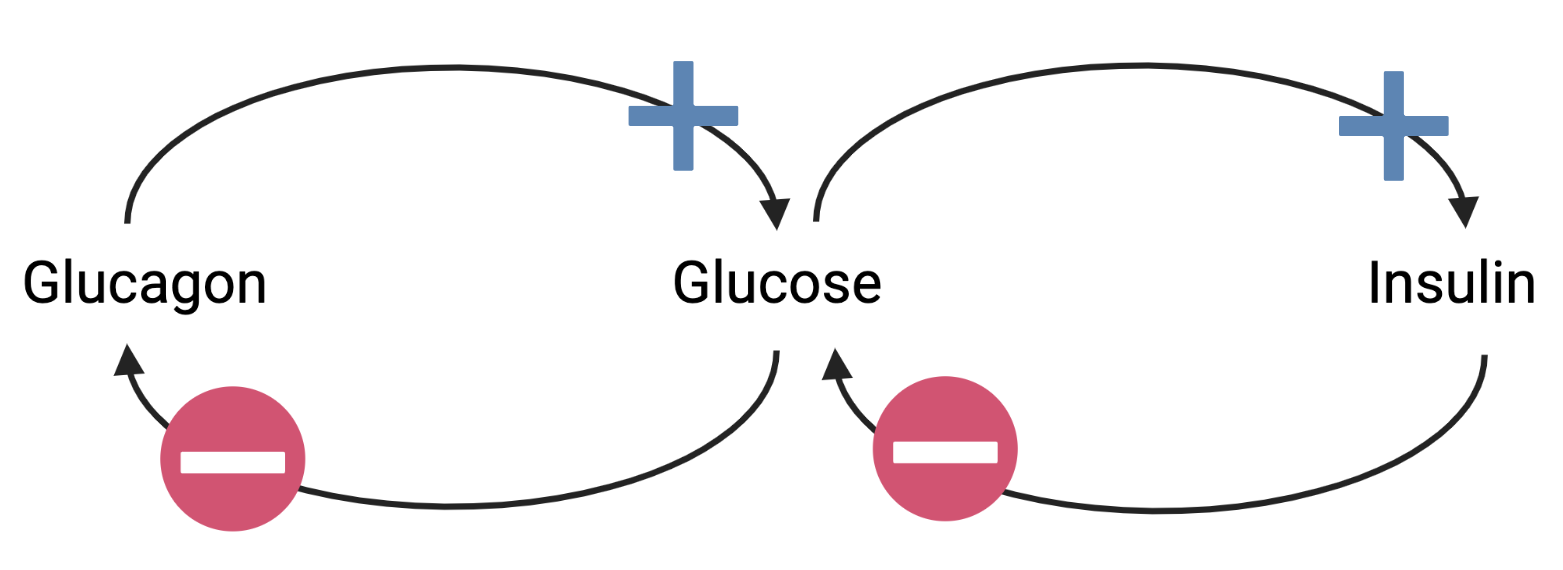
\includegraphics[width=1\linewidth]{./figure/glucose_homeo.png}
    \caption{Simple Model of Glucose Homeostasis that does not consider the organs or cellular mechanisms underlying the homeostatic relationship between the three components. In this system, glucose is being regulated. \footnotesize{(Created with BioRender.com)}}
    \label{fig:glucose_homeo}
\end{figure}

Figure \ref{fig:complete_glucose_homeo} below provides a more complete model of glucose regulation. It includes multiple mechanisms that glucose can be regulated and the role of metabolic organs such as the liver and the endocrine pancreas.

\begin{figure}[!ht]
    \centering
    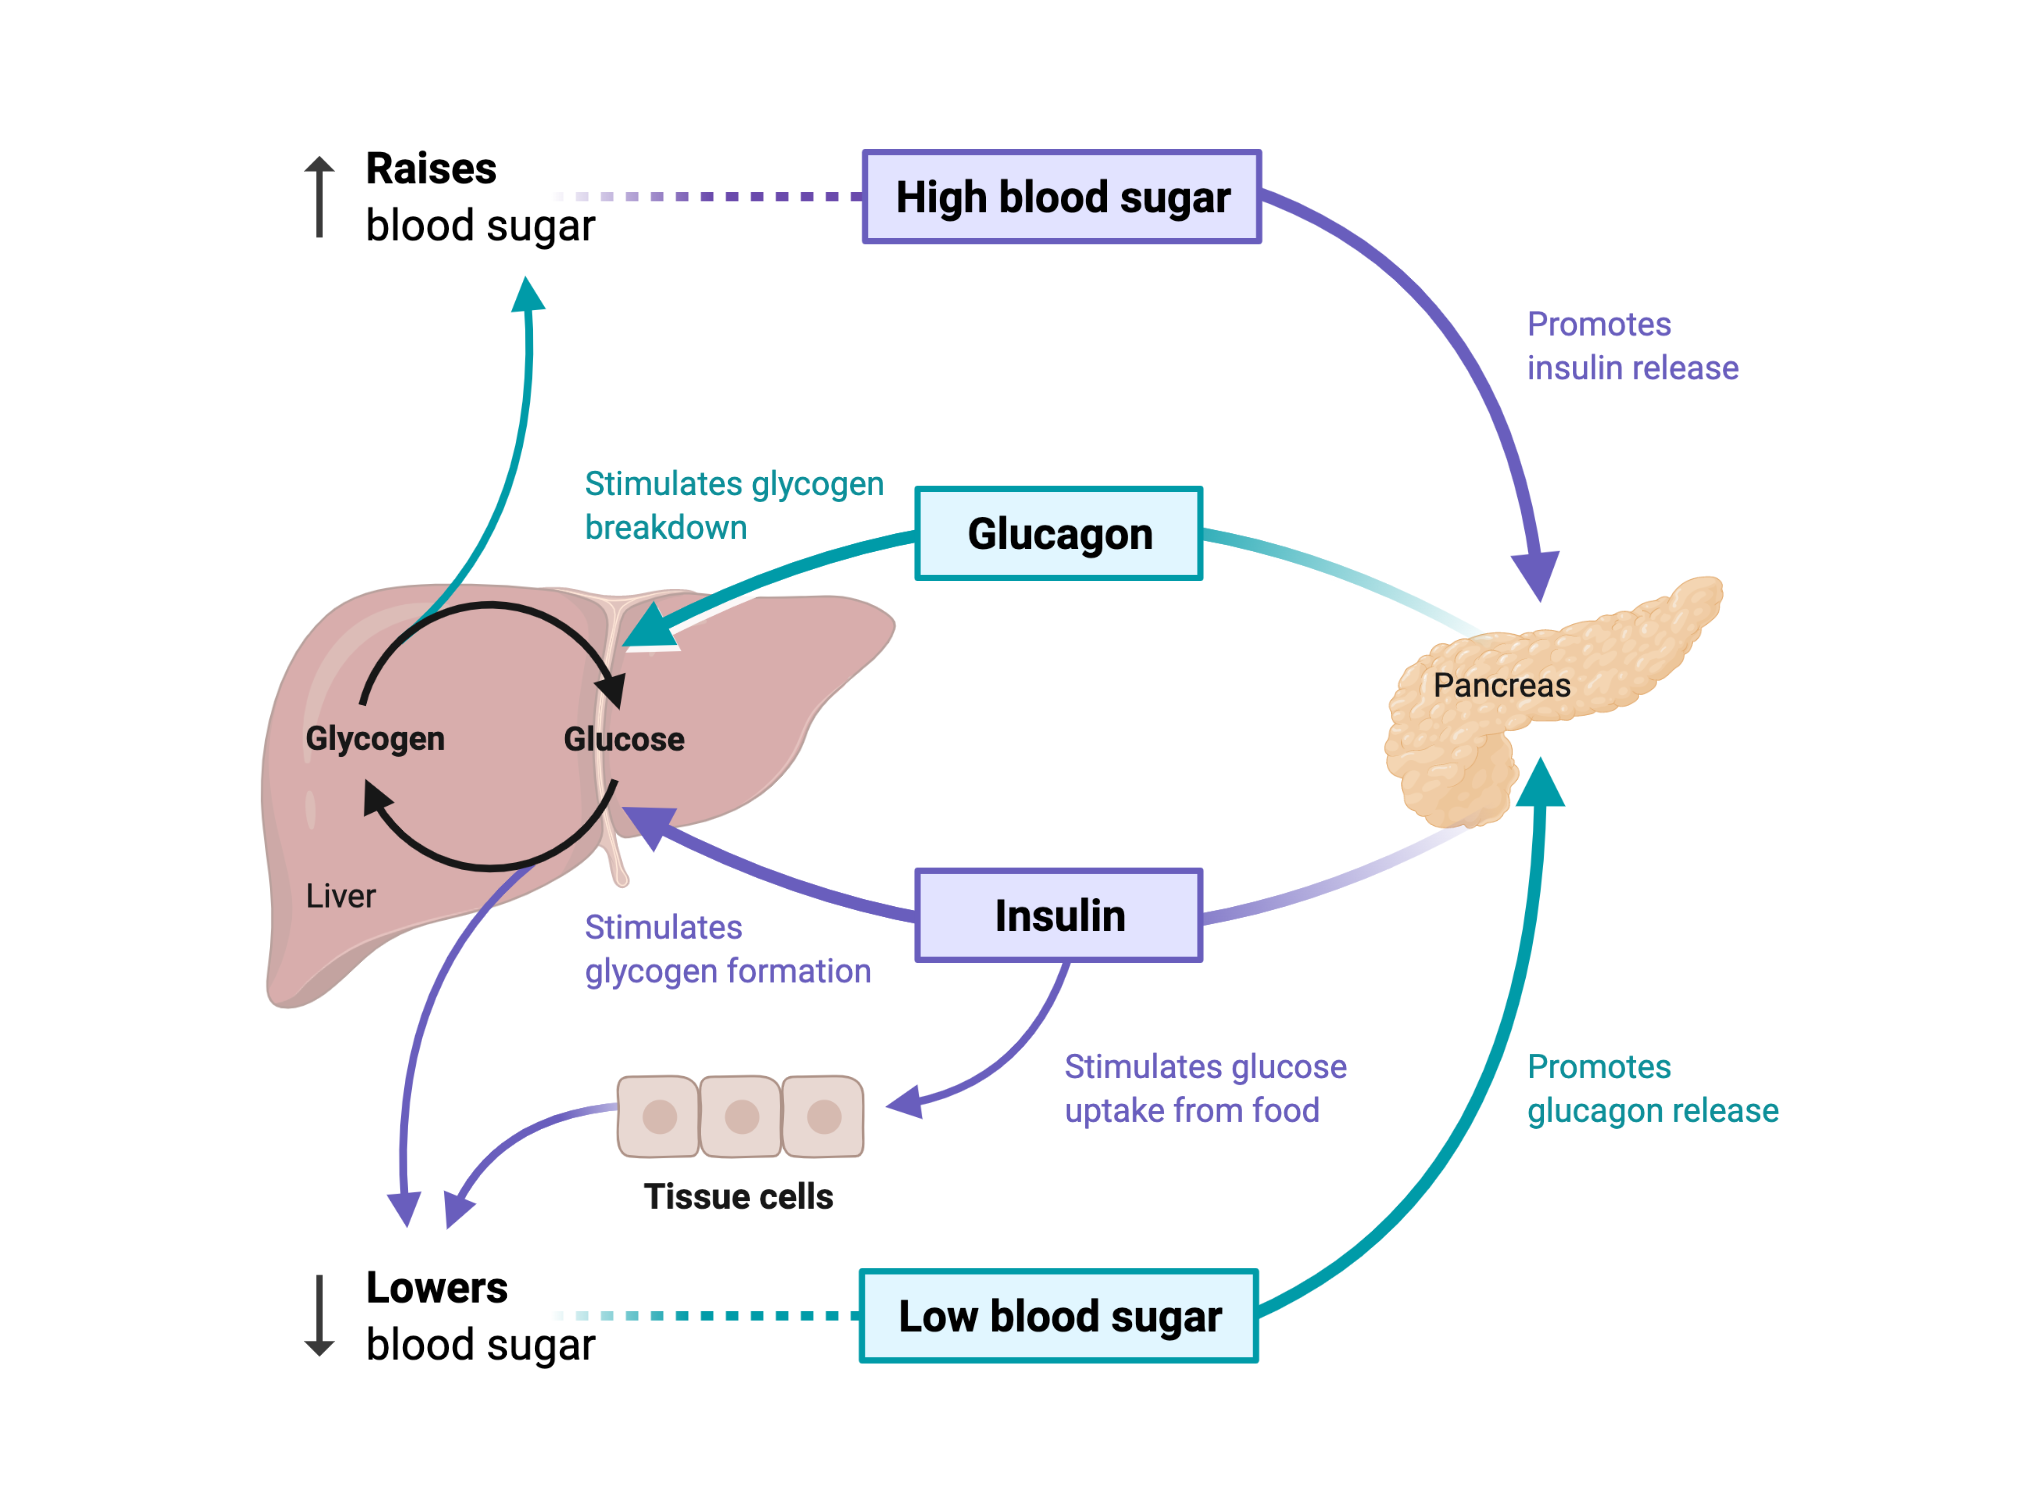
\includegraphics[width=1\linewidth]{./figure/complete_glucose_homeo.png}
    \caption{Model of Glucose Homeostasis that includes the organs involved in this homeostatic system \footnotesize{(Created with BioRender.com)}}
    \label{fig:complete_glucose_homeo}
\end{figure}

\paragraph{Analysis of Patient/Client Problems}
Homeostasis is routinely applied to the analysis of patient/client problems. Many diseases, conditions and syndromes, regardless of their underlying cause, results in some sort of disturbance to homeostasis; and thus any disturbance in homeostasis is ultimately analyzed for the possible causes.

\subsection{Interdependence}
Cells, tissues, organs, organ systems interact with one another (are dependent on the function of one another) to sustain life. Interdependence includes hierarchies of homeostatic regulation. The function and capacity of the whole system is related to the interdependent relationship between the parts, capabilities and attributes of each of the multiple systems. 

\paragraph{Analysis of Patient/Client Problems}
Interdependence is applied to the analysis of patient/client problems during the process of differential diagnosis. This process includes asking the question - "What are all the things that could cause this problem?" The list of possible causes can grow quickly given the interdependence of the whole system (the whole person).

\subsection{Structure - Function}
The function of a cell, tissue, or organ is determined by its form. Structure and function (from the molecular level to the organ system level) are intrinsically related to each other. Structure influences function (right now) and function influences structure (eventually). Part II is how muscle structure influences function right now. Part IV includes how function influences structure eventually (hypertrophy and atrophy).

\paragraph{Analysis of Patient/Client Problems}
Structure - Function is applied in the process of diagnosis of pathoanatomical conditions and also is the foundation for pathokinesiological interventions. If function is impaired, we consider the structure that may result in such an impaired function. For example, if there is an deviation in the gait pattern (function), we may consider the length of the hip flexors (structure impacts function). If there is a functional movement deviation, prolonged sitting (function), we may teach corrective exercises to prevent future changes in structure (shortened hip flexors) that become dysfunctions (function impacts structure eventually).

\subsection{Hierarchy of Adaptation}

A hierarchy of adaptation and adaptability works within and around physiological systems. Adaptation refers to changes that occur to the system so that it optimizes function. A muscle fiber creates tension. Adaptation refers to changes that occur so a muscle fiber can attain, sustain and maintain the ability to create tension. Adaptability refers to the ability to adapt. The hierarchy includes genetic, epigenetic, anatomic, physiologic, behavioral and cultural changes. Cultural changes being a mechanism of passing behavioral adaptation from one generation to another. This entire hierarchy is involved through the life span and has relevance to physiological adaptation. Physiological adaptation includes genetic, epigenetic, anatomic, physiologic mechanisms and include changes to structure and function. Behaviors are enabled by our physiology, but then also influence our physiology (our physiology allows us to eat sugar, and then our eating of sugar influences our physiology). And the culture around us gives rise to acceptable, and not acceptable, behaviors. 

\paragraph{Analysis of Patient/Client Problems}
Physical therapists incorporate the hierarchy of adaptation with the World Health Organization's International Classification of Function (ICF), see Figure \ref{fig:icf}. The ICF is a model that describes how physiological systems contribute (as body systems and functions) and interact with functioning (or dysfunction or impairments). The ICF model focuses on the bidirectional interactions between bodily functions (and structures), activities (movements and behaviors) and participation (behaviors and interactions). It also considers to health conditions that impact functions, activities and participation along with external and personal factors. 

\begin{figure}[!ht]
    \centering
    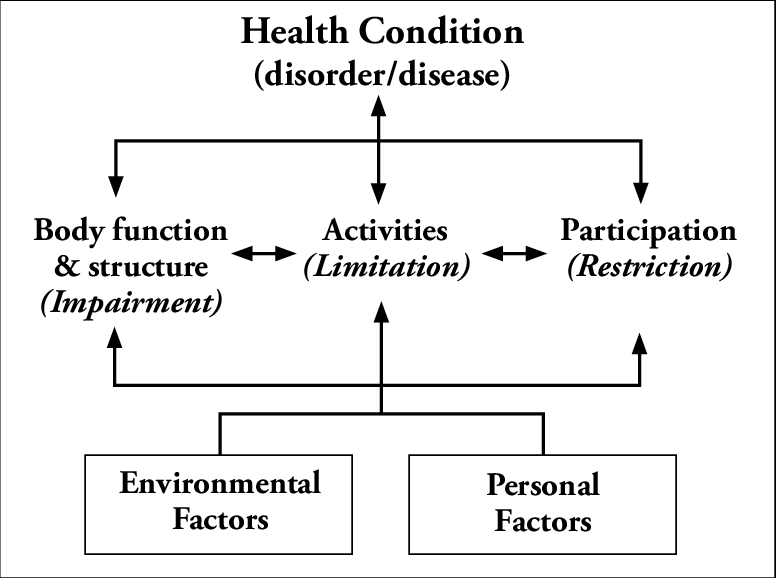
\includegraphics[width=1\linewidth]{./figure/ICF.png}
    \caption{International Classification of Function (ICF) \footnotesize{(Created with BioRender.com)}}
    \label{fig:icf}
\end{figure}

The ICF is useful for understanding physiological interdependence, structure - function relationships, and the hierarchy of adaptation. The middle of the ICF is \textit{Activity}, which is primarily referring to movement, making the ICF a movement centered approach. The model considers what is necessary for movement, body structure and functions; and why we do movements, to participate. In this way the ICF overlaps with our muscle centered approach as depicted in Figure \ref{fig:muscle_centered_approach_icf}

\begin{figure}[!ht]
    \centering
    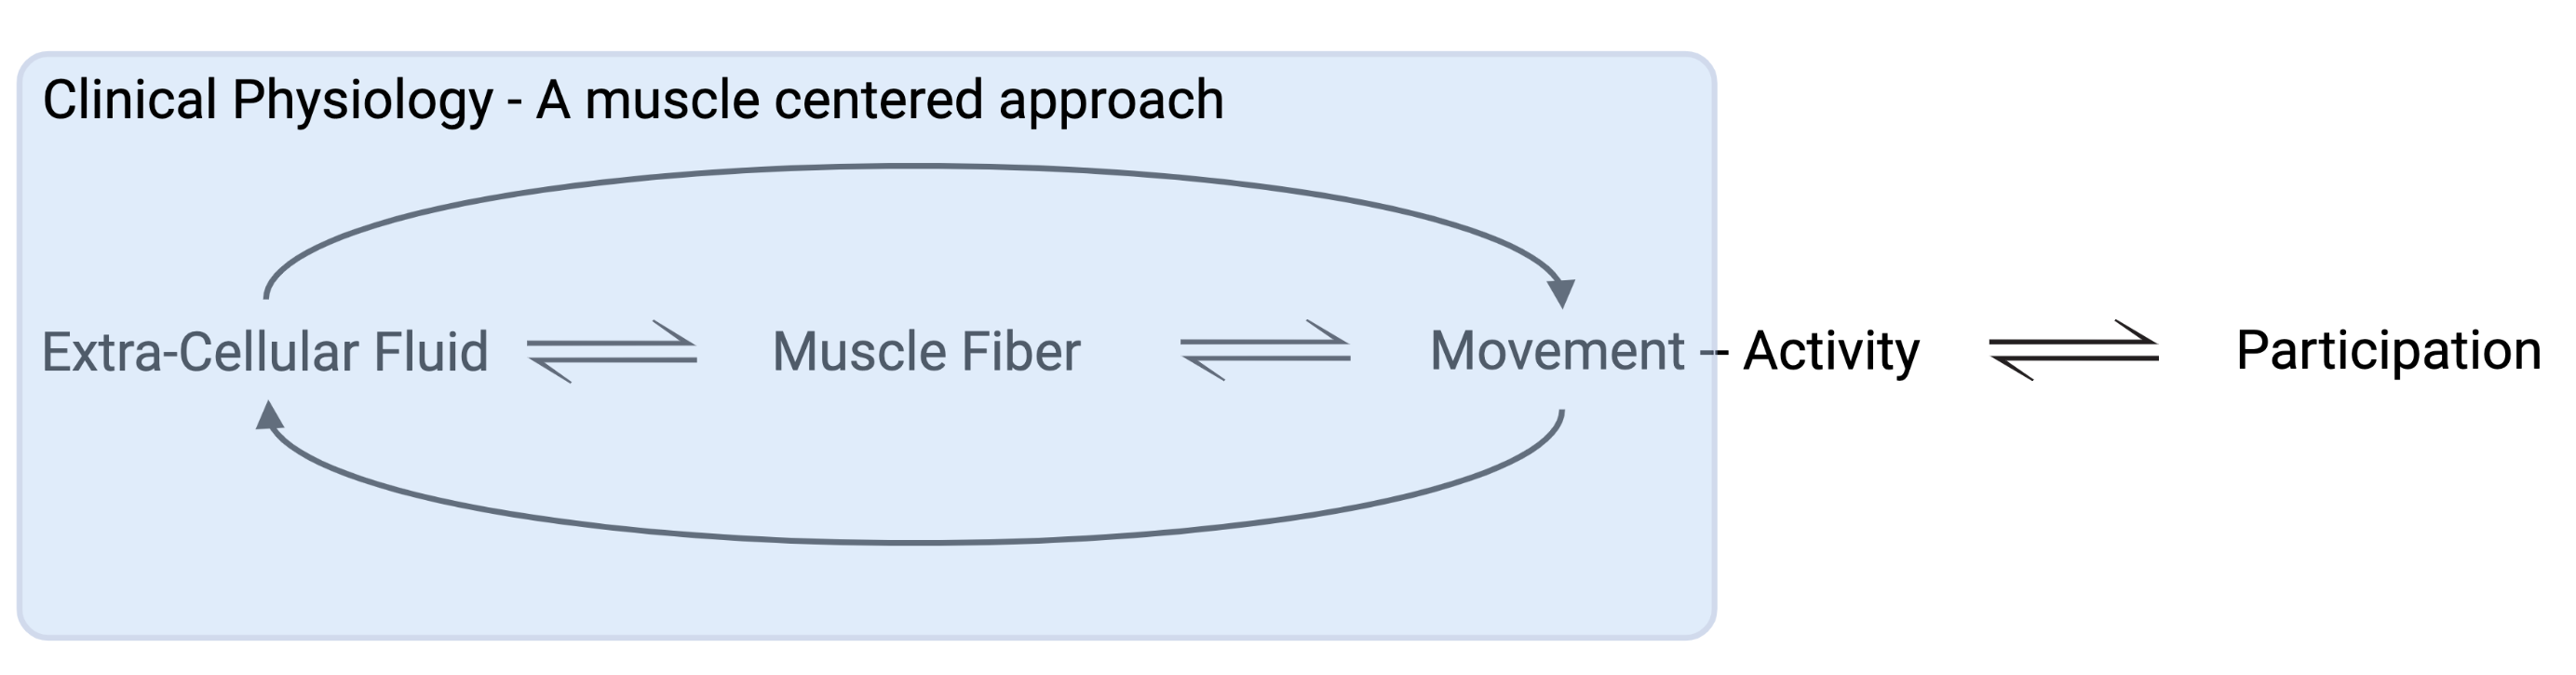
\includegraphics[width=1\linewidth]{./figure/muscle_centered_approach_icf.png}
    \caption{Muscle centered approach overlap with the ICF \footnotesize{(Created with BioRender.com)}}
    \label{fig:muscle_centered_approach_icf}
\end{figure}

\section{Chapter Summary \& Next Steps}

A muscle centered approach to clinical physiology for a physical therapist is based on the relationship between muscle fibers, movement and extra-cellular fluid. Muscle fibers are necessary, but not sufficient, causes of movement. Movement is a multi-system physiological function and contributes to the ECF (Figure \ref{fig:muscle_centered_approach}). Therefore, movement is critical to the health and well-being of the body since it is critical to the ECF, and the ECF is critical to all cells. The muscle centered approach is a \textit{middle out}\cite{noble_music_2008} approach to understanding the complexity and hierarchy of physiology for the physical therapist as a movement specialist. By \textit{middle out} we refer to the entire approach as a model of clinical physiology that looks upward in scale (movement as a behavior within a culture) and looking downward in scale (to the genes).

\paragraph{Next Steps}
In Chapter \ref{chp:fundamentals} on Fundamentals we review muscle \textit{in situ} including the muscle scaffold including connective tissue, tendons and bony attachments. This flows into some movement considerations such as attaining and sustaining tension, active and passive tension, and muscle organization and arrangement. It is important to have a foundation of these fundamentals for understanding the behavior of muscles \textit{in situ} that muscle fibers contribute and the bidirectional implications of the muscle - muscle fiber relationship in causing movement.

\printbibliography[heading=subbibintoc]